\subsubsection*{Inicialización de la MMU}

\par Para administrar la memoria en el área libre contamos con un contador de páginas inicializado en la dirección 0x00100000. A medida que el sistema necesita una página,  éste contador se incrementa en 4K, como muestra la siguiente implementación:

\begin{lstlisting} [caption={Contador de Páginas Libres}],label=mmucontador] 
void * siguiente_libre;

void inicializar_mmu()
{
  siguiente_libre = (void *) PAGE_COUNTER_INIT;
}

void * dar_siguiente()
{
    uint i;
    for(i = 0; i<1024; i++) ((pde *) siguiente_libre)[i].present = 0;
    siguiente_libre += 0x1000;
    return siguiente_libre - 0x1000;
}
\end{lstlisting}

\par Al crear una página, recorremos todas entradas de la tabla seteando el bit de presente en 0 (sea ésta un directorio o tabla de páginas). Para simplificar la manipulación en el código de las pde y pte creamos dos estructuras en C correspondientes a las ya mencionadas: 

\begin{lstlisting} [caption={struct Page Directory Entry}],label=mmupde] 
typedef struct pde_t {
    unsigned char present:1;
    unsigned char read_write:1;
    unsigned char user_supervisor:1;
    unsigned char page_level_write_through:1;
    unsigned char page_level_cache_disable:1;
    unsigned char accessed:1;
    unsigned char reserved:1;
    unsigned char page_size:1;
    unsigned char global:1;
    unsigned char available_9_11:3;
    unsigned int  base_address:20;
} __attribute__((__packed__, aligned (4))) pde;
\end{lstlisting}

\begin{lstlisting} [caption={struct Page Table Entry}],label=mmupte] 
typedef struct pte_t {
    unsigned char present:1;
    unsigned char read_write:1;
    unsigned char user_supervisor:1;
    unsigned char page_level_write_through:1;
    unsigned char page_level_cache_disable:1;
    unsigned char accessed:1;
    unsigned char dirty:1;
    unsigned char page_table_attribute_index:1;
    unsigned char global:1;
    unsigned char available_9_11:3;
    unsigned int  base_address:20;
} __attribute__((__packed__, aligned (4))) pte;
\end{lstlisting}

\subsubsection*{Mapeo y Desmapeo de Páginas}

\par \texttt{mmu_mapear_pagina} toma una dirección lineal virtual, una dirección física, un directorio de tablas de página, y dos chars para indicar read/write y user/supervisor. La rutina realiza lo siguiente:
\begin{itemize}
\item (1) Se fija si el pde indicado por los 10 bits más significativos de la dirección lineal está presente en el directorio de páginas pasado por parámetro.
\item  (2) Si no está presente, crea una tabla de páginas con los atributos pasados por parámetro, y modifica la pde correspondiente en el directorio, para que apunte a ella.
\item (3) Luego, modifica la pte indicada por los siguientes 10 bits más significativos, como indica la figura, de la tabla creada (o modifica la ya existente en caso en que estaba en presente), cambiando el base address por la dirección física pasada por parámetro, corrida 12 bits correspondientes al offset, ya que las páginas están alineadas a 4k. El offset para buscar un dato dentro de ellas está en los 12 bits menos significativos de la dirección lineal.
\end{itemize}
\begin{figure}[ht!]
\centering
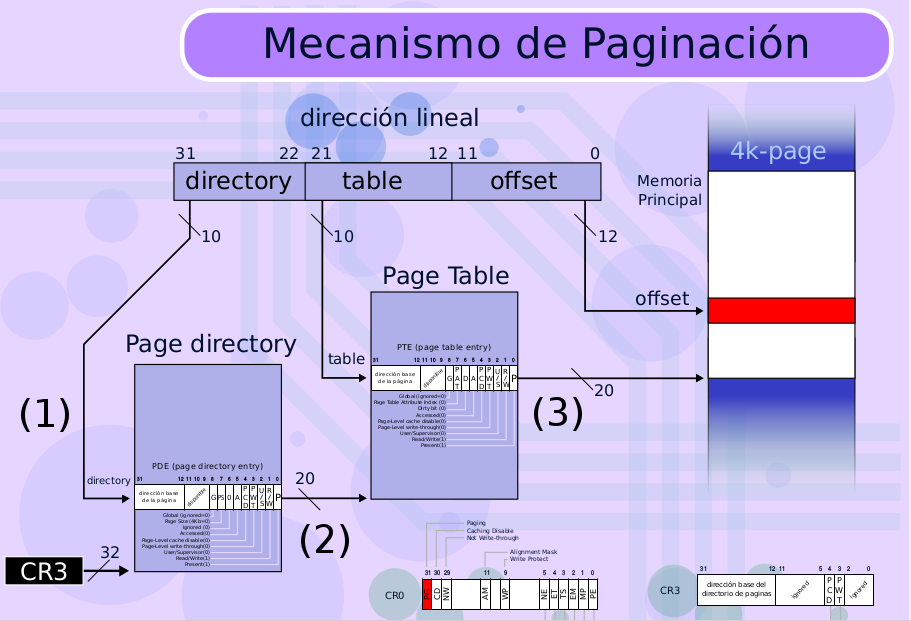
\includegraphics[width=100mm]{imagenes/paginacion.png}
\caption{Mapeo de Páginas}
\end{figure}

\par Análogamente, \texttt{mmu_unmapear_pagina} toma una dirección lineal y un directorio de tablas de página, y lo que hace es buscar primero la pde correspondiente en el directorio, indicado por los 10 bits más significativos, luego en dicha tabla busca la pte indicada por los siguientes 10 bits de la dirección lineal, y coloca el bit de presente de dicha entrada en 0.

\par Por la construcción del kernel, las direcciones de los mapas de memoria están mapeadas con indentity mapping. Como en estas funciones se modifica el directorio y/o tablas de páginas, al final se llama a \texttt{tlbflush() }para que se invalide la cache de traducción de direcciones. 

\subsubsection*{Inicialización de directorios y tablas para Tareas Pirata}

\par La rutina \texttt{mmu_inicializar_dir_pirata} se encarga de inicializar un directorio de páginas y tablas de páginas para una tarea, respetando la organización de la memoria establecida por el enunciado como muestra la siguiente figura:

\begin{figure}[ht!]
\centering
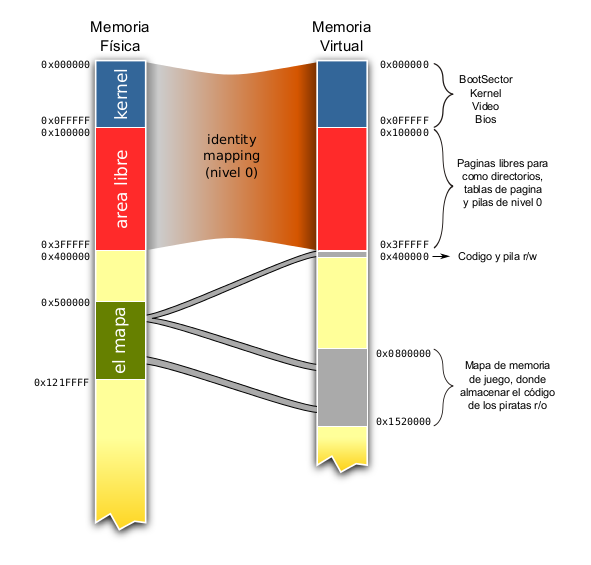
\includegraphics[width=100mm]{imagenes/memoriatarea.png}
\caption{Mapa de memoria de la Tarea.}
\end{figure}

\par Para lograr esto, la función toma como parámetros el jugador, el pirata y los parámetros que escribirá en la pila y luego utilizará la tarea. La rutina realiza lo siguiente:
\begin{itemize}
\item Obtenemos una página nueva usando la función previamente mencionada \texttt{dar_siguiente} para el directorio, y otra para la tabla de páginas del kernel. La tabla del kernel la inicializamos con la función \texttt{mmu_inicializar_tabla_kernel_para_pirata}, que básicamente hace una copia de la original, mapeando con identiy mapping las direcciones 0x00000000 a 0x003FFFFF como fue explicado en el ejercicio 3.

\item La primera entrada del directorio de páginas de la tarea se completa con la dirección base de la tabla de kernel inicializada en el item anterior, con los bits de read/write en 0, presente en 1, user/supervisor en 0 y reserved en 0, ya que sólo será accedido por las interrupciones del sistema de nivel 0, y sólo será de lectura.

\item Mapeamos las páginas de las posiciones exploradas del jugador entre las posiciones 0x0800000 y 0x1520000 como indica la figura. Para ello, recorremos la matriz de posiciones del mapa, y para aquellas que hayan sido exploradas por el jugador, calculamos su indice de página y mapeamos a la dirección correspondiente usando la función \texttt{mmu_mapear_pagina}.
\begin{lstlisting} [caption={Mapeo de páginas de posiciones exploradas.}],label=mmudirpirata1] 
 for(i = 0; i<MAPA_ALTO; i++){
     for(j = 0; j<MAPA_ANCHO; j++){
     	if(jugador->posiciones_exploradas[i][j]){
                uint ind = (i*MAPA_ANCHO+j) * 0x1000;
                mmu_mapear_pagina(0x800000+ind, resultado, 0x500000+ind, 0, 1);
            }
        }
    }
\end{lstlisting}

\item Mapeamos usando nuevamente \texttt{mmu_mapear_pagina} en la dirección virtual 0x400000 del directorio de la tarea, la dirección física correspondiente a la posición inicial del pirata, es decir, el puerto de donde sale. Dicha dirección se calcula usando la función auxiliar dada \texttt{game_xy2lineal}, que dada la posición inicial del pirata (la tenemos guardada en un array en cada struct del jugador), devuelve el índice de la página de memoria física a partir de la dirección 0x500000 correspondiente a esa posición del mapa.
\begin{lstlisting} [caption={Mapeo de la página correspondiente a la posición inicial.}],label=mmudirpirata2] 
mmu_mapear_pagina(0x400000, resultado, game_xy2lineal(p[0],p[1])*0x1000+0x500000, 1, 1);
\end{lstlisting}

\item Por último, queda copiar el código de la tarea correspondiente a la página de la posición inicial del pirata (mapeada en el paso anterior en el directorio del pirata en la dirección 0x400000). Para eso, como en el momento en que creamos un pirata estamos en el contexto del kernel, necesitamos mapear antes dicha posición al directorio del kernel. Elegimos mapearla también en la dirección 0x400000 (se hace análogamente al ítem anterior, pero en el directorio del kernel ubicado en la dirección 0x27000). Una vez hecho esto, copiamos el código de la tarea (se encuentra en las posiciones 0x10000 para A-E, 0x11000 para A-M, 0x12000 para B-E y 0x13000 para B-M, según qué jugador y qué tipo de pirata sea) usando la función auxiliar \texttt{copiar_pagina}, que copia cada elemento de los 4K de memoria. Además, escribimos en la pila (ubicada en la misma página que el código, al final) los parámetros que luego usará dicha tarea.

\item La función retorna el directorio de páginas de la tarea pirata.

\end{itemize}

\par 













